% --------------------- VARIABLEN -------------------------

\newcommand{\COURSE}{Physik und Materialwissenschaften\\ Praktikum Physik \\}
\newcommand{\SEMESTER}{Elektro- und Informationstechnik II}
\newcommand{\STUDENT}{Maximilian Spahn\\ und\\Benjamin Langer}

\newcommand{\HEADDING}{Praktikum Physik}
\newcommand{\SUBHEADDING}{Versuch 3.2: pn-Übergang und Solarzelle}

% ------------------- DEFINITIONEN -----------------------

\documentclass[a4paper]{scrartcl}

\usepackage[utf8]{inputenc}
\usepackage[ngerman]{babel}
\usepackage{amsmath}
\usepackage{amssymb}
\usepackage{color}
\usepackage{tikz}
\usepackage{float}
\usetikzlibrary{arrows,decorations.markings}
\usepackage{tabularx}
\usepackage{fancybox}
\usepackage{pgfplots}
\usepackage{geometry}
\usepackage{fancyhdr}
\usepackage[page]{totalcount}
\usepackage[colorlinks=true,linkcolor=black,urlcolor=blue,bookmarks,bookmarksopen=true]{hyperref}

%Größe der Ränder setzen
\geometry{a4paper,left=2cm, right=2cm, top=3cm, bottom=2cm, headheight=8cm}

%Kopf- und Fußzeile
\pagestyle {fancy}
\fancyhf{}
\fancyhead[L]{\STUDENT}
\fancyhead[C]{\COURSE}
\fancyhead[R]{\today}

\fancyfoot[L]{\SEMESTER}
\fancyfoot[C]{}
\fancyfoot[R]{Seite \thepage /\pageref{LastPage}}

%Formatierung der Überschrift, hier nichts ändern
\def\header#1#2{
  \begin{center}
    {\Large #1}\\
    {#2}
  \end{center}
}

\numberwithin{equation}{subsection}

\setlength\parindent{0pt}

% ----------------------- DOCUMENT ---------------------------

\begin{document}

\vspace{10pt}
\header{\HEADDING}{\SUBHEADDING}

\tableofcontents

\newpage

\section{Einleitung}
In der folgenden Ausarbeitung wird die Funktionsweise einer Solarzelle anhand des Versuches
\glqq pn-Übergang und Solarzelle\grqq \hspace{0cm} messtechnisch untersucht. Der Versuch behandelt
den Unterschied einer unbeleuchteten und einer beleuchteten Solarzelle. Die Ergebnisse werden graphisch
und rechnerisch ausgewertet.
\newpage
\section{Theorie}
%TODO
TODO

\newpage
\section{Häusliche Vorarbeit}
\subsection{An welchen Stellen des I-U Diagramms wird eine höhere Dichte an Messwerten benötigt?}
Am Anfang der Kennlinie von $-2V$ bis $0V$ ist der Verlauf relativ linear. Dadurch werden theoretisch nur
zwei Messwerte und praktisch nur wenige Messwerte benötigt. Das liegt daran, dass die Diode für diesen
Fall in Sperrrichtung geschaltet ist und die Spannung am parallelgeschalteten Widerstand $r_{\text{sh}}$
abfällt (siehe Abbildung \ref{fig:ESB_Solar}). Ab $0V$ wird die Diode nicht mehr in Sperrrichtung sondern
in Flussrichtung geschaltet, wodurch der Anteil des Stromes der durch die Diode fließt zunimmt.
Da die Kennlinie der Diode exponentiell verläuft und der größte Teil der Spannung nun an der Diode
abfällt, muss die Anzahl der Messwerte deutlich erhöht werden.

\begin{figure}[H]
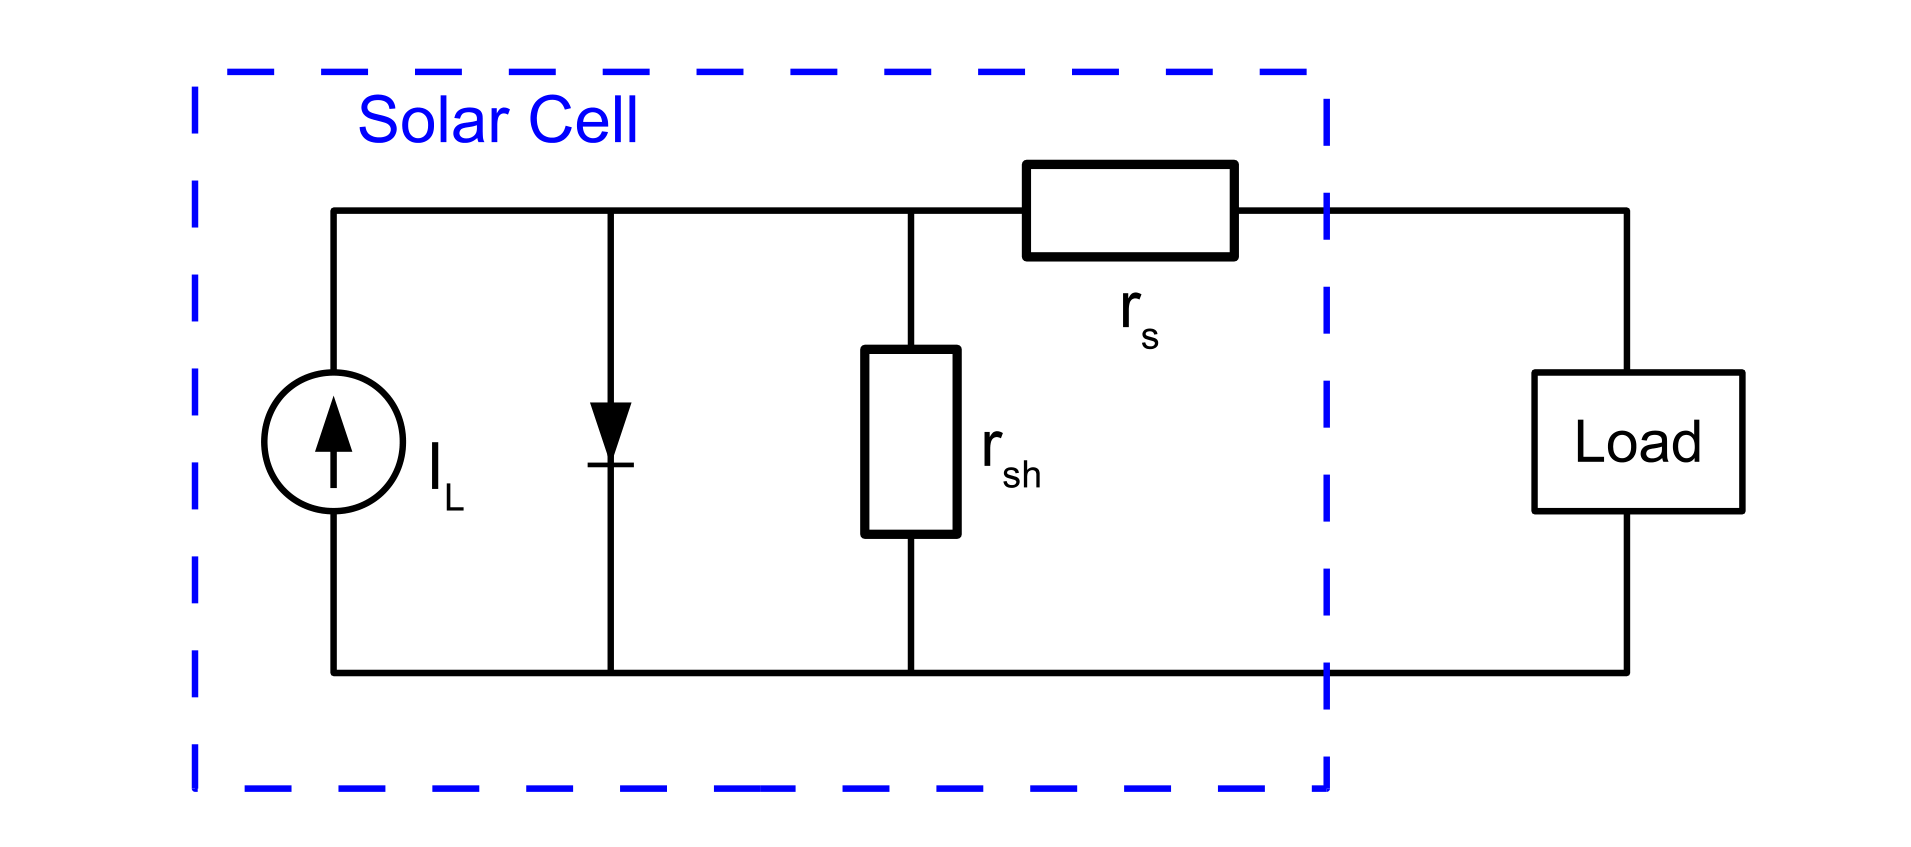
\includegraphics[width=16cm]{ESB_Solarzelle}
\centering
\caption{Ersatzschaltbild der Solarzelle}
\centering
\label{fig:ESB_Solar}
\end{figure}

\subsection{I-U Diagramme für eine unbeleuchtete und beleuchtete Solarzelle}

\begin{figure}[H]
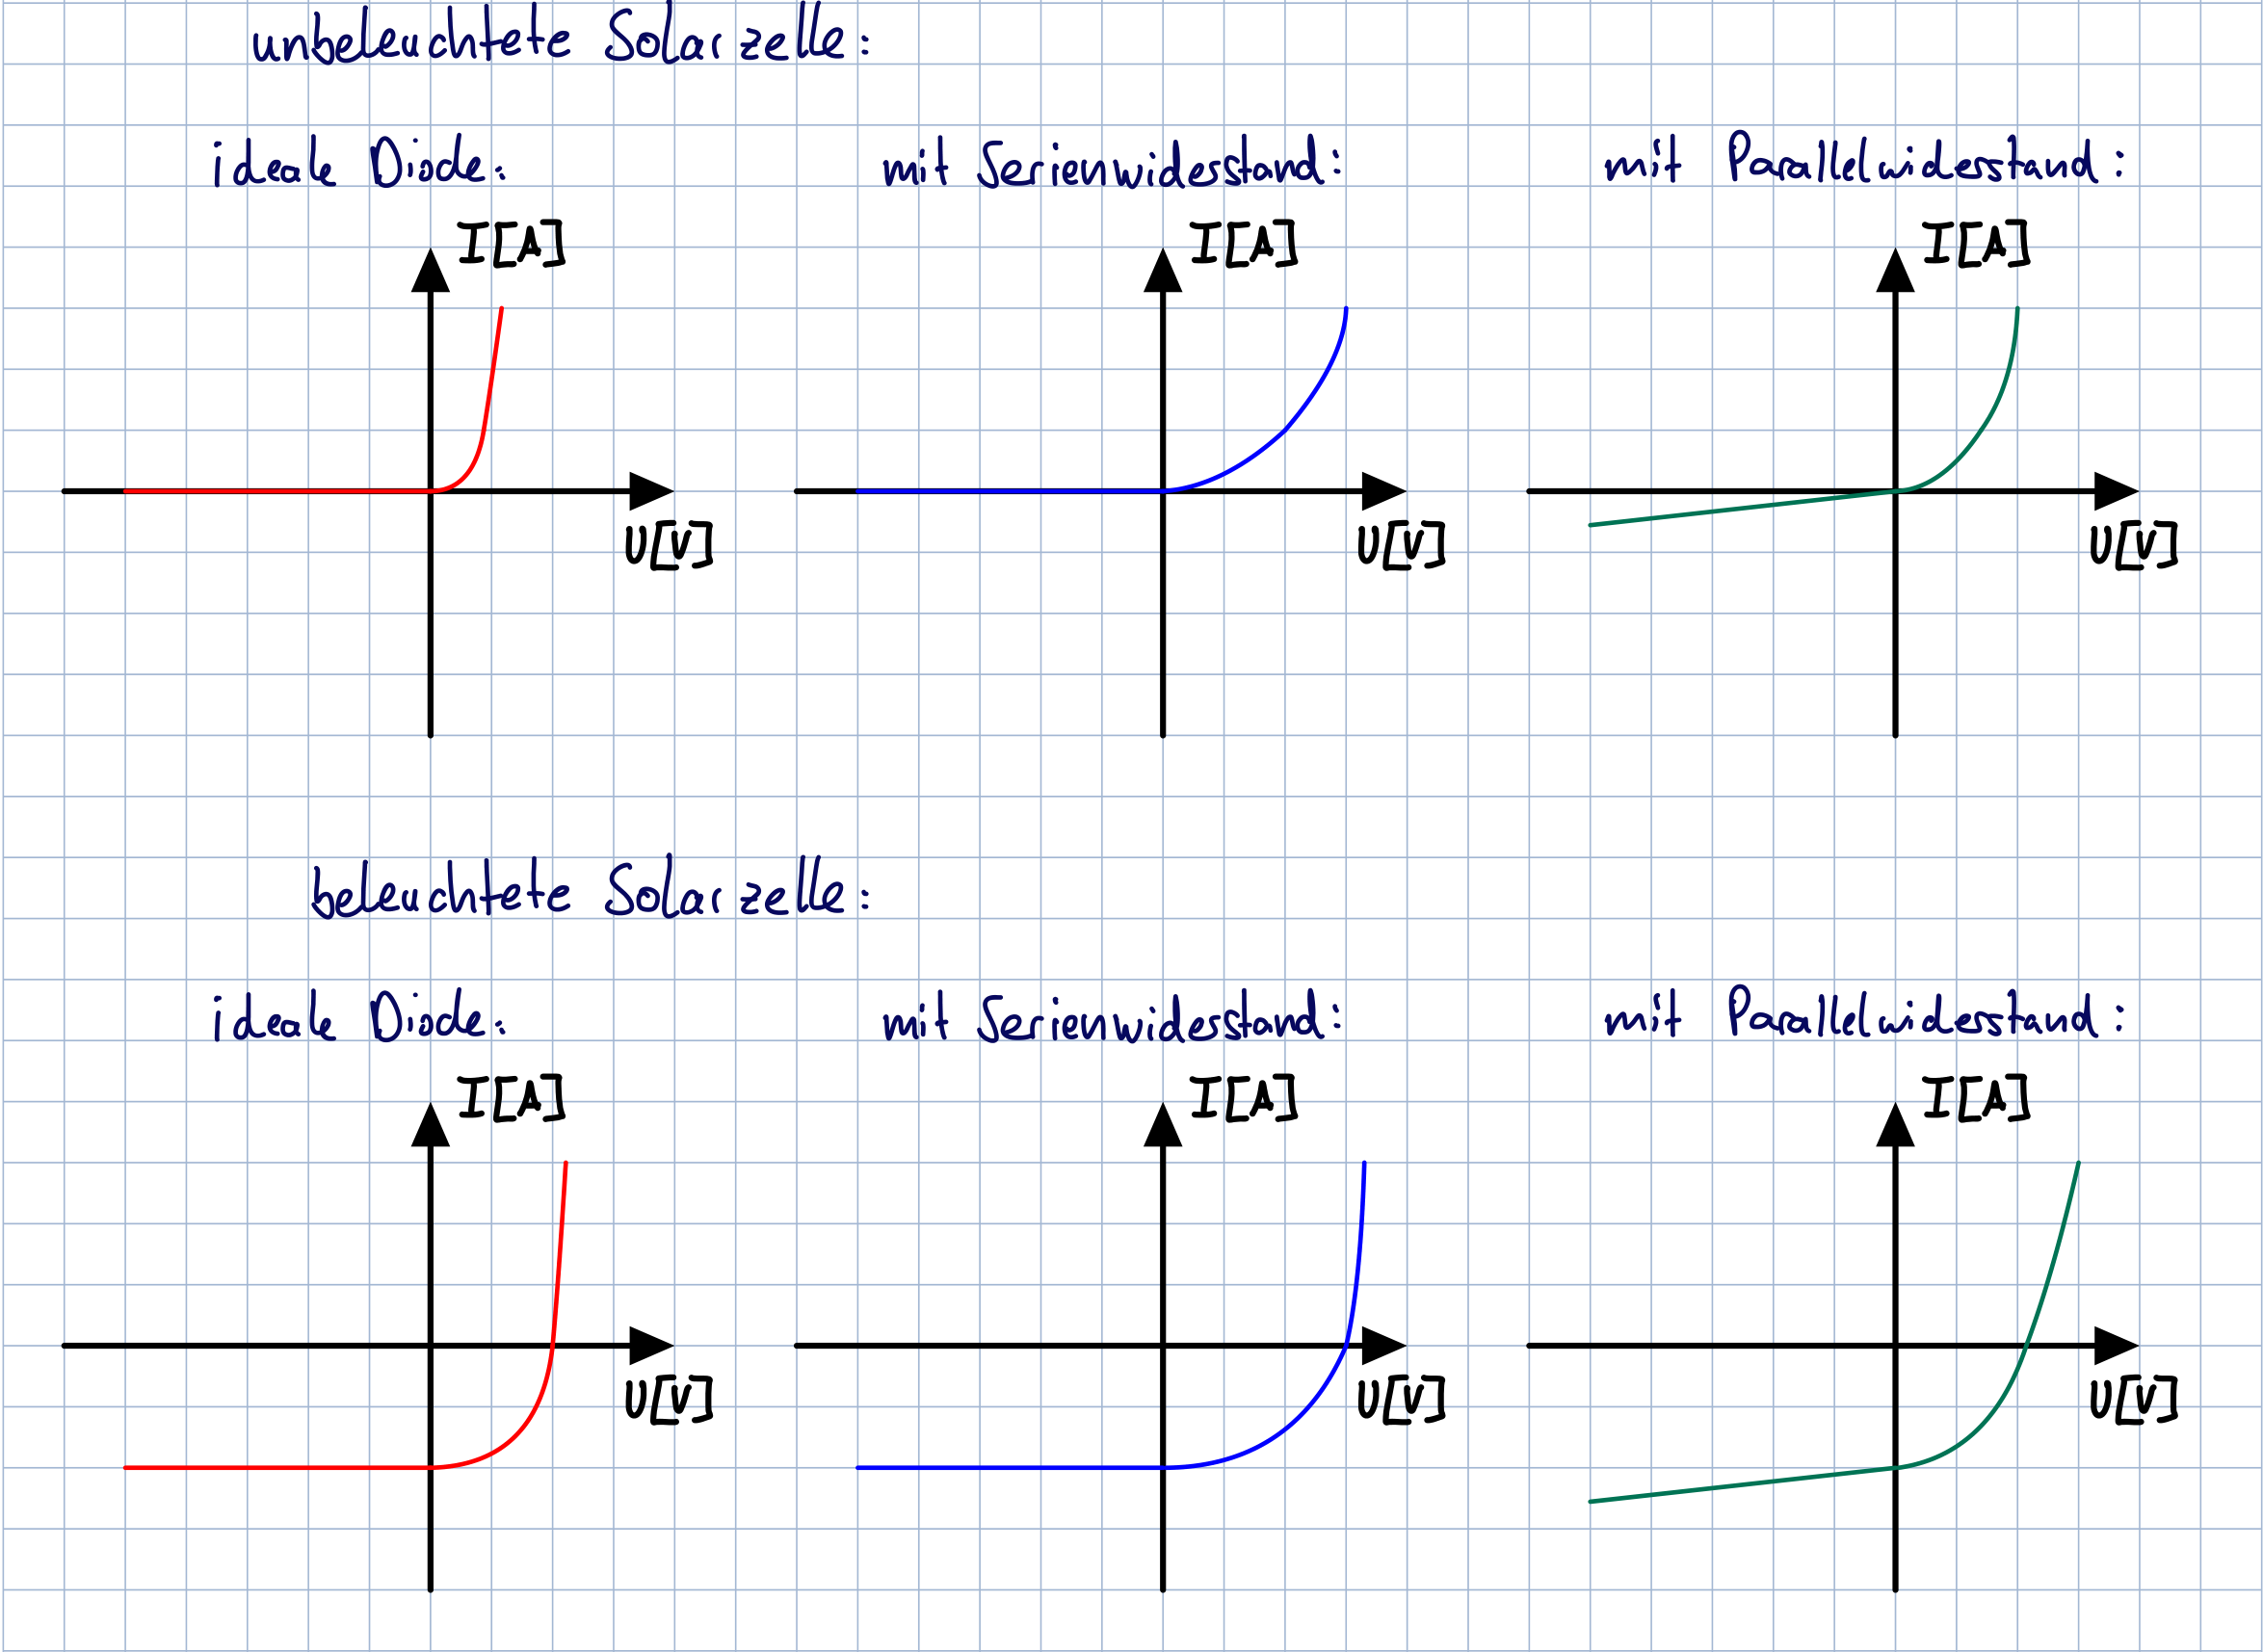
\includegraphics[width=16cm]{Kennlinie}
\centering
\caption{Kennlinien für beleuchtete- und unbeleuchtete Solarzelle}
\centering
\label{fig:Kennlinien}
\end{figure}

\subsection{Einfluss der Widerstände auf den Füllfaktor}
Je größer der Füllfaktor wird, desto mehr ähnelt die Kennlinie einer idealen Stromquelle. Das heißt die
Solarzelle wird effizienter, je näher der Füllfaktor am Wert 1 liegt. Dies wäre der Fall, wenn
der Serienwiderstand gegen 0 $\lim_{r_{\text{s}} \to 0}$ und der Parallelwiderstand gegen unendlich ginge
$\lim_{r_{\text{sh}} \to \infty}$ (siehe Abbildung \ref{fig:ESB_Solar}).

\subsection{Aktueller Stand der Technik bei Solarzellen}
Solarzellen bestehen zum größten Teil aus p-dotiertem und n-dotiertem Silizium.
Es wird vor Allem wegen der hohen Verfügbarkeit auf der Erde verwendet.
Man unterscheidet zwischen polykristallinen- und monokristallinen Zellen.
Polykristalline Zellen werden aus Silizium gegossen und haben einen Wirkungsgrad
von 12-16\%. Monokristalline Zellen werden aus gezüchtetem Silizium gebaut, wodurch die Herstellung
teurer ist. Dafür wird ein höhere Effizienzvon 14-20\% erreicht. Der typische Füllfaktor liegt
zwischen 0,5 und 0,7.
%TODO Quellenverweis.

\newpage
\section{Aufbau und Durchführung}
\subsection{Aufbau}
Der Versuchsaufbau ist in Abbildung \ref{fig:Aufbau} dargestellt.

\begin{figure}[H]
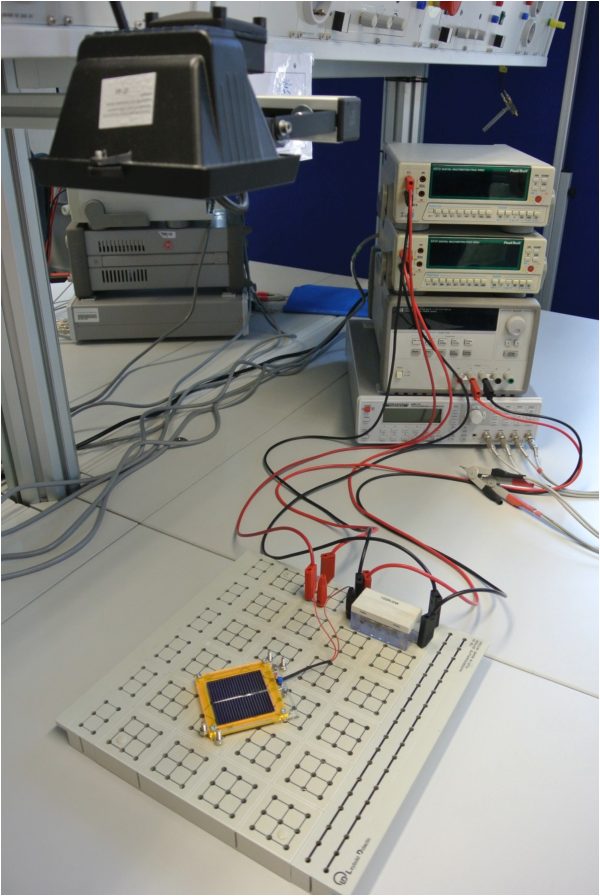
\includegraphics[width=14cm]{Aufbau}
\centering
\caption{Versuchsaufbau}
\centering
\label{fig:Aufbau}
\end{figure}

\subsection{Durchführung}
Die Schaltung wird wie in Abbildung \ref{fig:Schaltplan} zu sehen
aufgebaut. Zuerst wird der Versuch mit abgedeckter Solarzelle durchgeführt. Man misst für verschiedene
Spannungen $U_d$ von $-2,0V$ bis $0,6V$ die Spannung $U_R$. Dadurch lässt sich der Diodenstrom $I_d$
berechnen. Mit den Strom- und Spannungswerten lässt sich nun die U-I Kennlinie der Diode zeichnen. Danach 
wird der Versuch nochmal mit beleuchteter Solarzelle wiederholt.

\begin{figure}[H]
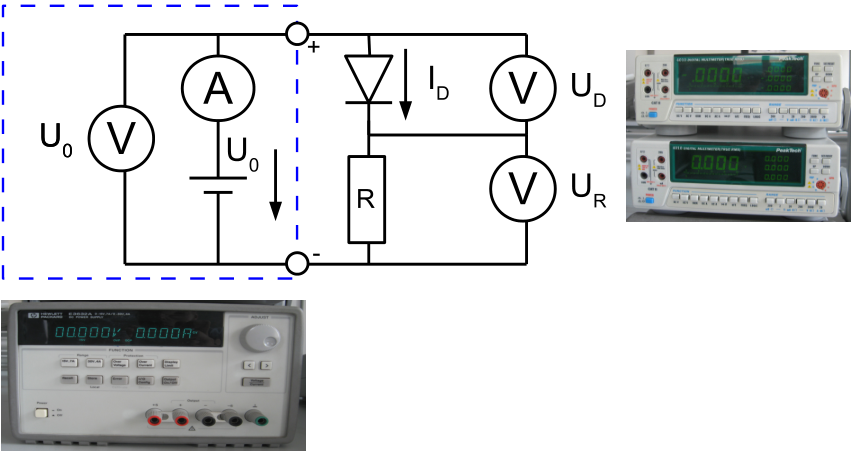
\includegraphics[width=16cm]{Schaltplan}
\centering
\caption{Schaltplan}
\centering
\label{fig:Schaltplan}
\end{figure}

\newpage
\section{Auswertung Versuch}
Die Kapazität $C_s$ beträgt: $924,63\;nF$. Die Standardabweichung wird
auf $1\;nF$ geschätzt.

\begin{align*}
C_s = (925,0\pm 1,0)\;nF	
\end{align*}

Die Solarzelle hat eine quadratische Grundfläche $A$ mit einer Seitenlänge (l)
von $(52,5\pm 0,5)\;mm$.

\begin{align*}
A &= l^2 \\
 &= (52,5\;mm)^2 \\
 &= 2756,25\;mm^2
\end{align*}

\begin{align}
\frac{\partial A}{\partial l} = 2l
\end{align}

\begin{align*}
U_a = \bigg | \frac{\partial A}{\partial l} \bigg | \cdot U_l = 52,5\;mm^2 \\
A = (2756\pm 53)\;mm^2
\end{align*}

Die Kapazität eines Plattenkondensators mit gegebenem $\epsilon_r = 11,9$ lässt sich berechnen mit:
\begin{align*}
C &= \epsilon_0 \cdot \epsilon_r \cdot \frac{A}{d} \\
d &= \epsilon_0 \cdot \epsilon_r \cdot \frac{A}{C} \\
  &= 8,854 \cdot 10^{-12}\; \frac{As}{Vm} \cdot 11,9 \cdot \frac{2756,26 \; mm^2}{924,64 \; nF} \\
  &= 314,082 \; nm 
\end{align*}

\begin{align}
&\frac{\partial d}{\partial A} = \epsilon_0 \cdot \epsilon_r \cdot \frac{1}{C}
&\frac{\partial d}{\partial C} = - \epsilon_0 \cdot \epsilon_r \cdot \frac{A}{C^2}
\end{align}

\begin{align*}
U_d = \bigg | \frac{\partial d}{\partial A} \bigg | \cdot U_A + \bigg | \frac{\partial d}{\partial C} 
\bigg | \cdot U_C = 6,3222 \; nm
\end{align*}
\begin{align*}
d = (314,1 \pm 6,4)\; nm
\end{align*}

Folgende Größen lassen sich in der Abbildung \ref{fig:beleuchtet} oder der Tabelle \ref{tab:beleuchtet} im 
Anhang (Abschnitt \ref{sec:Anhang}) ablesen:
\begin{align*}
&\text{Die Leerlaufspannung}\; U_{OC} \; \text{beträgt:} &&0,52\;V \\
&\text{Der Kurzschulssstrom}\; I_{SC} \; \text{beträgt:} &-&0,064333\;A \\
&\text{Die maximale Leistung}\; P_{max} \; \text{beträgt:} &-&0,024296\;W\\
\end{align*}

Der Füllfaktor lässt sich durch die Gleichung \ref{} berechnen:
\begin{align*}
FF = \frac{-0,024296\;W}{0,52\;V \cdot (-0,064333\;A)} = 0,72625
\end{align*}
\\
Messunsicherheit Multimeter geschätzt:
\begin{align*}
U_M = \pm 0,01\;V
\end{align*}
\begin{align*}
U_{OC} = (0,52 \pm 0,01)\;V \\
U_R = (-9,65 \pm 0,01)\;V
\end{align*}

Messunsicherheit vom Widerstand $R_{SC}$:
\begin{align*}
R = (150 \pm 10)\; \Omega \\
\end{align*}

Die Messunsicherheit für $I_{SC}$ berechnet sich wie folgt:
\begin{align*}
I_{SC} = \frac{U_R}{R}
\end{align*}

\begin{align}
&\frac{\partial I_{SC}}{\partial U_R} = \frac{1}{R}
&\frac{\partial I_{SC}}{\partial R} = - \frac{U_R}{R^2}
\end{align}

\begin{align*}
U_{I_{SC}} = \bigg | \frac{\partial I_{SC}}{\partial U_R} \bigg | \cdot U_{U_R} +
\bigg | \frac{\partial I_{SC}}{\partial R} \bigg | \cdot U_R = 0,0043\overline{5} \; A
\end{align*}
\begin{align*}
I_{SC} = (-0,0643 \pm 0,0044)\; A
\end{align*}

Die Messunsicherheit für $P_{max}$ berechnet sich wie folgt:
\begin{align*}
P_{max} = U_{OC} \cdot I_{SC}
\end{align*}

\begin{align}
&\frac{\partial P_{max}}{\partial U_{OC}} = I_{SC}
&\frac{\partial P_{max}}{\partial I_{SC}} = U_{OC}
\end{align}

\begin{align*}
U_{P_{max}} = \bigg | \frac{\partial P_{max}}{\partial U_{OC}} \bigg | \cdot U_{U_{OC}} +
\bigg | \frac{\partial P_{max}}{\partial I_{SC}} \bigg | \cdot U_{I_{SC}} = 0,0029313 \; W
\end{align*}
\begin{align*}
P_{max} = (-0,0243 \pm 0,0030)\; W
\end{align*}

Die Messunsicherheit für den Füllfaktor $FF$ berechnet sich wie folgt:

\begin{align}
\frac{\partial FF}{\partial P_{max}} = \frac{1}{U_{OC} \cdot I_{SC}} \qquad
\frac{\partial FF}{\partial U_{SC}} = -\frac{P_{max}}{U_{SC}^2 \cdot I_{SC}} \qquad
\frac{\partial FF}{\partial I_{SC}} = -\frac{P_{max}}{U_{SC} \cdot I_{SC}^2}
\end{align}

\begin{align*}
U_{FF} = \bigg | \frac{\partial FF}{\partial P_{max}} \bigg | \cdot U_{P_{max}} +
\bigg | \frac{\partial FF}{\partial U_{SC}} \bigg | \cdot U_{U_{SC}} +
\bigg | \frac{\partial FF}{\partial I_{SC}} \bigg | \cdot U_{I_{SC}} = 0,1533
\end{align*}
\begin{align*}
FF = (0,73 \pm 0,16)
\end{align*}

\newpage
\section{Wertung/Fazit}
Der aus den Messwerten berechnete Füllfaktor liegt mit Ungenauigkeit im realistischen
Bereich. Durch die von uns sehr klein gewählte Schrittweite der Messwerte ist es uns
gelungen eine nah an der Theorie liegende U-I Kennlinie zu zeichnen.
Das Ergebnis des Versuchs ist alles in allem zufriedenstellend.


\newpage
\section{Anhang}
\label{sec:Anhang}
\begin{table}[H]
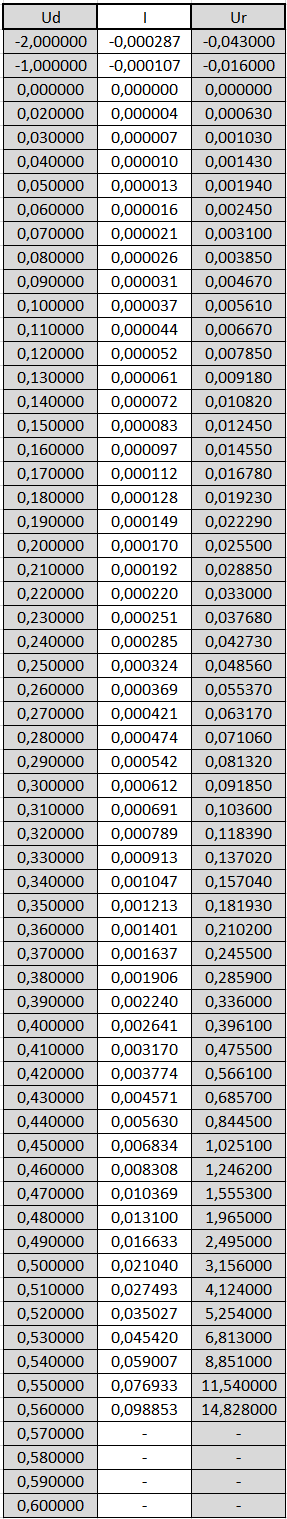
\includegraphics[width=4cm]{Tabelle_unbeleuchtet}
\centering
\caption{Messwerte Solarzelle unbeleuchtet}
\end{table}

\begin{figure}[H]
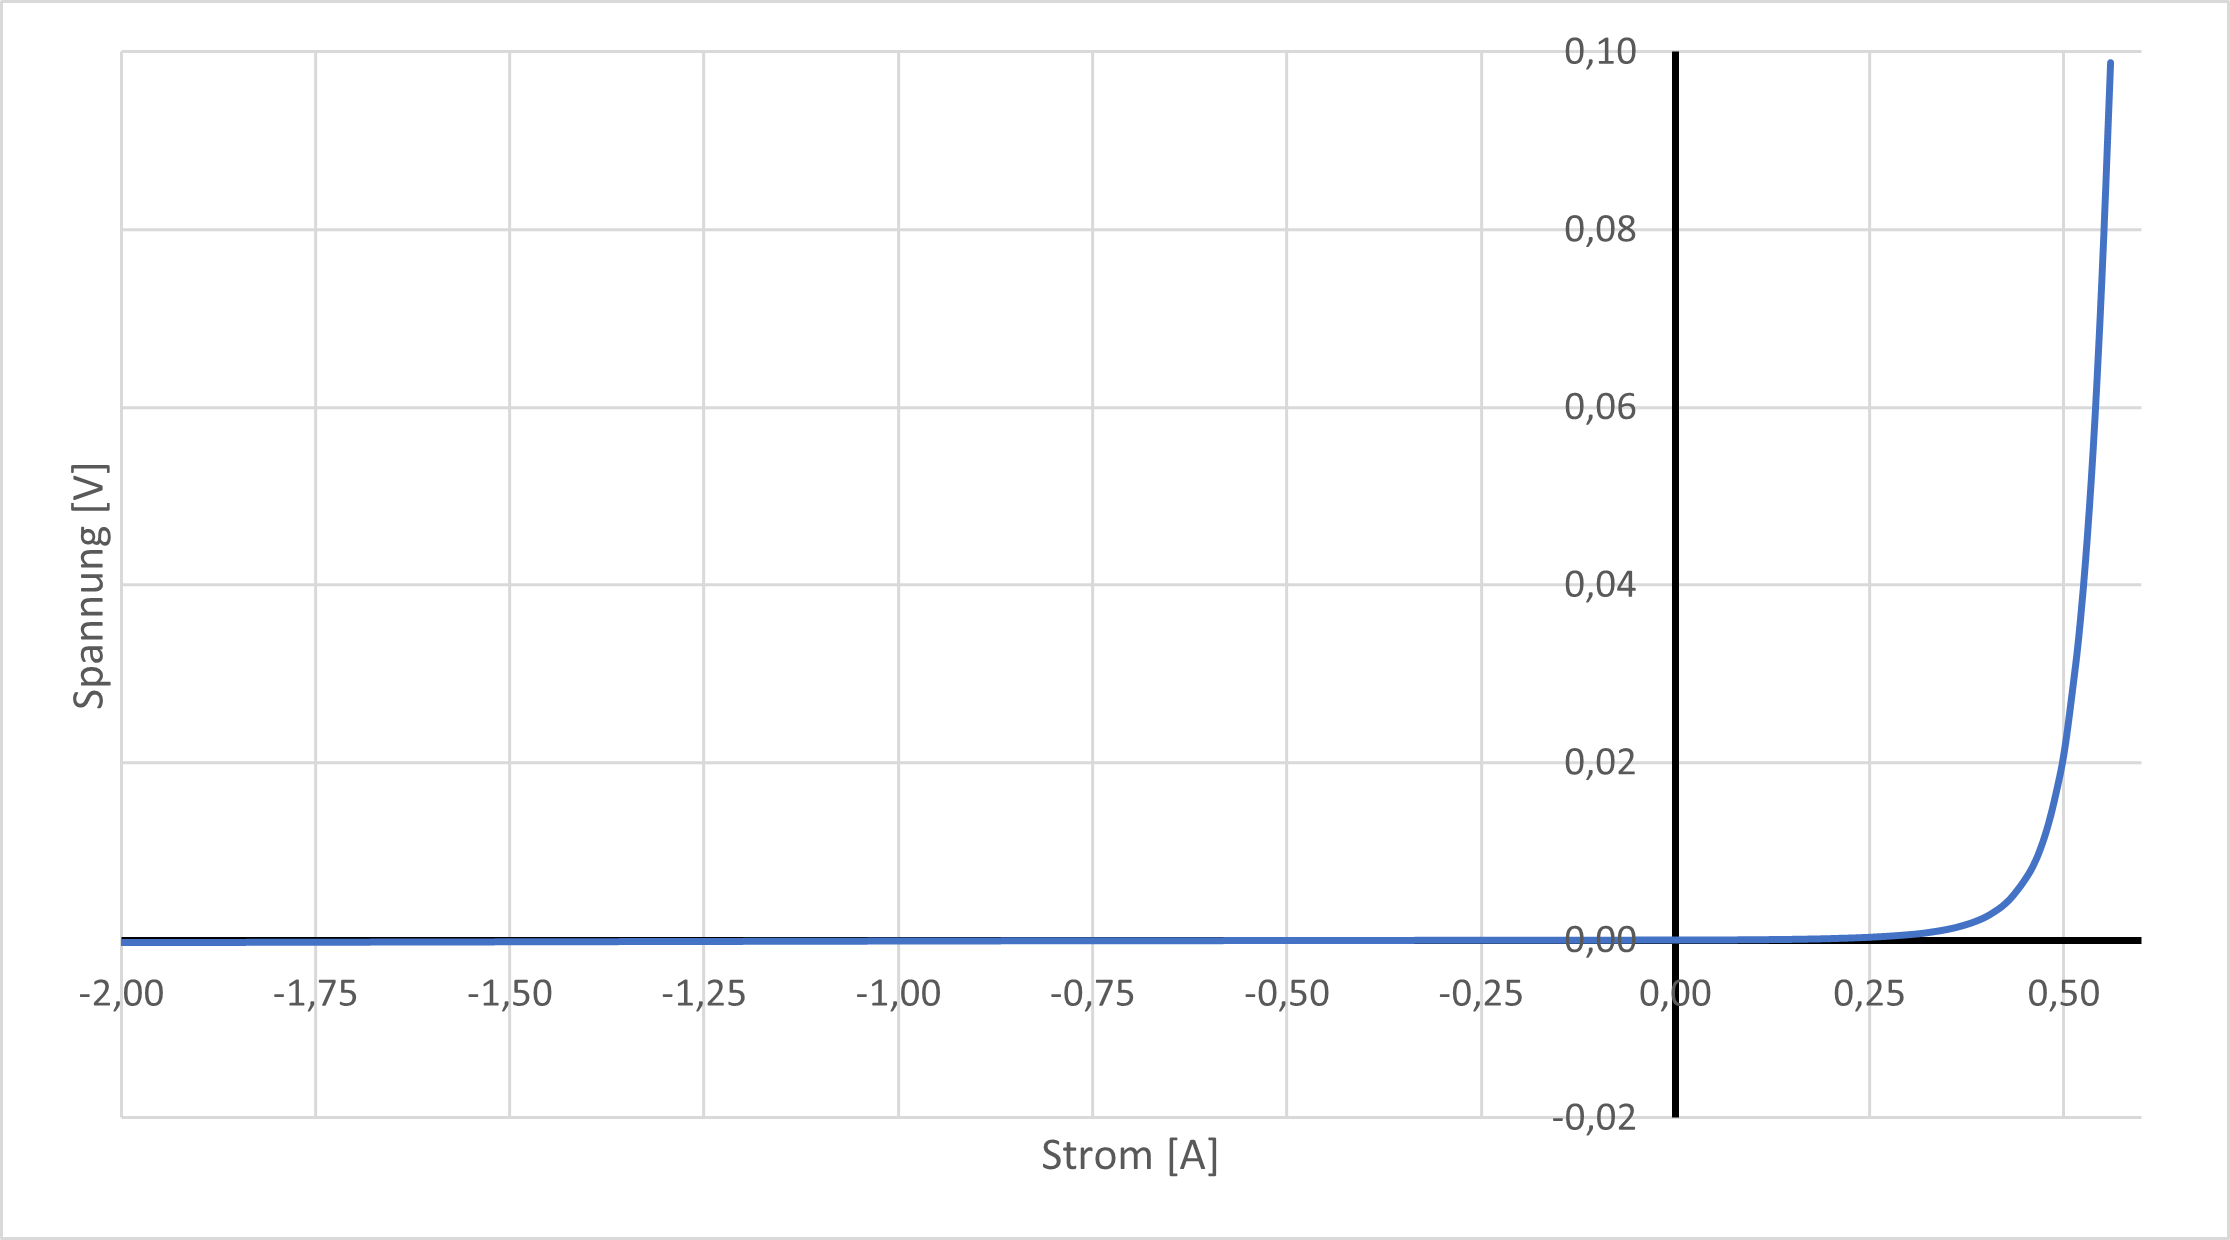
\includegraphics[width=14cm]{Diagramm_unbeleuchtet}
\centering
\caption{Diagramm Solarzelle unbeleuchtet}
\centering
\end{figure}

\begin{table}[H]
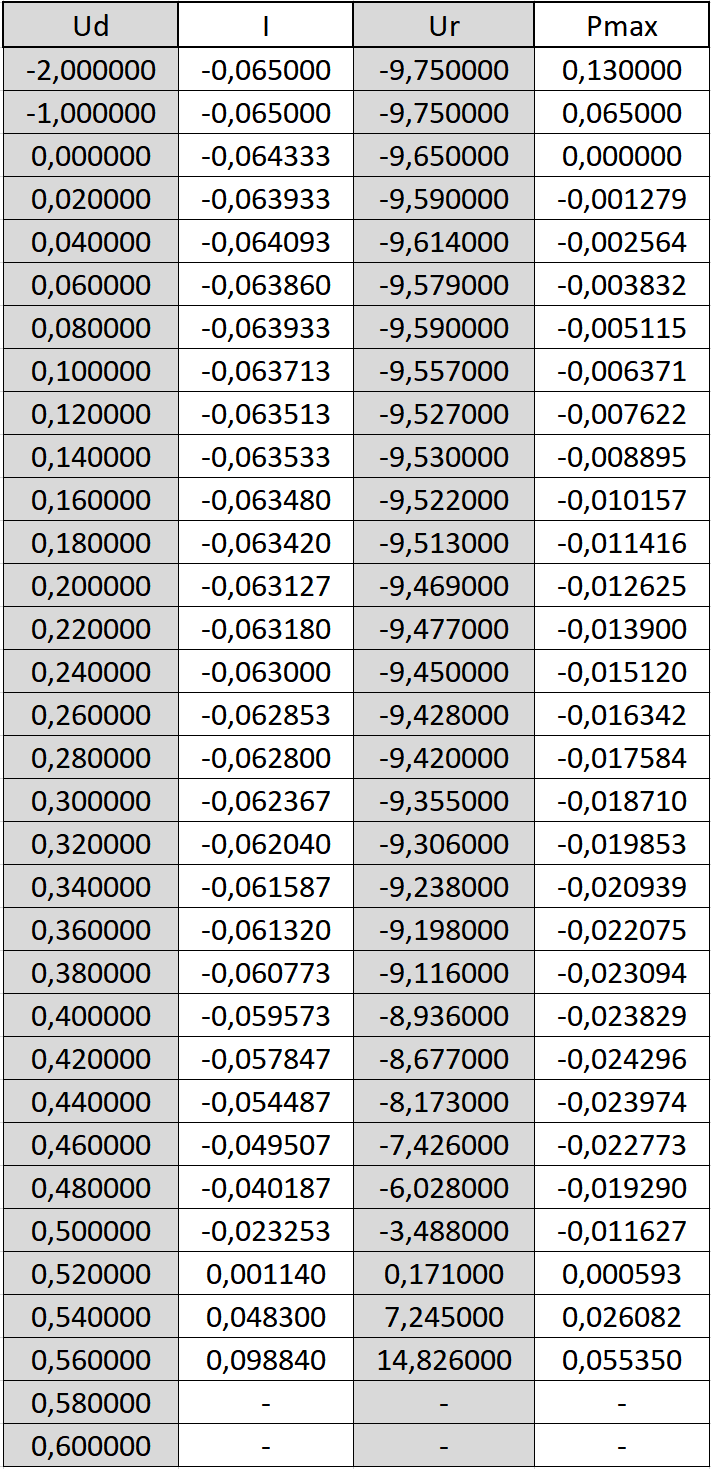
\includegraphics[width=6cm]{Tabelle_beleuchtet}
\centering
\caption{Messwerte Solarzelle unbeleuchtet}
\label{tab:beleuchtet}
\end{table}

\begin{figure}[H]
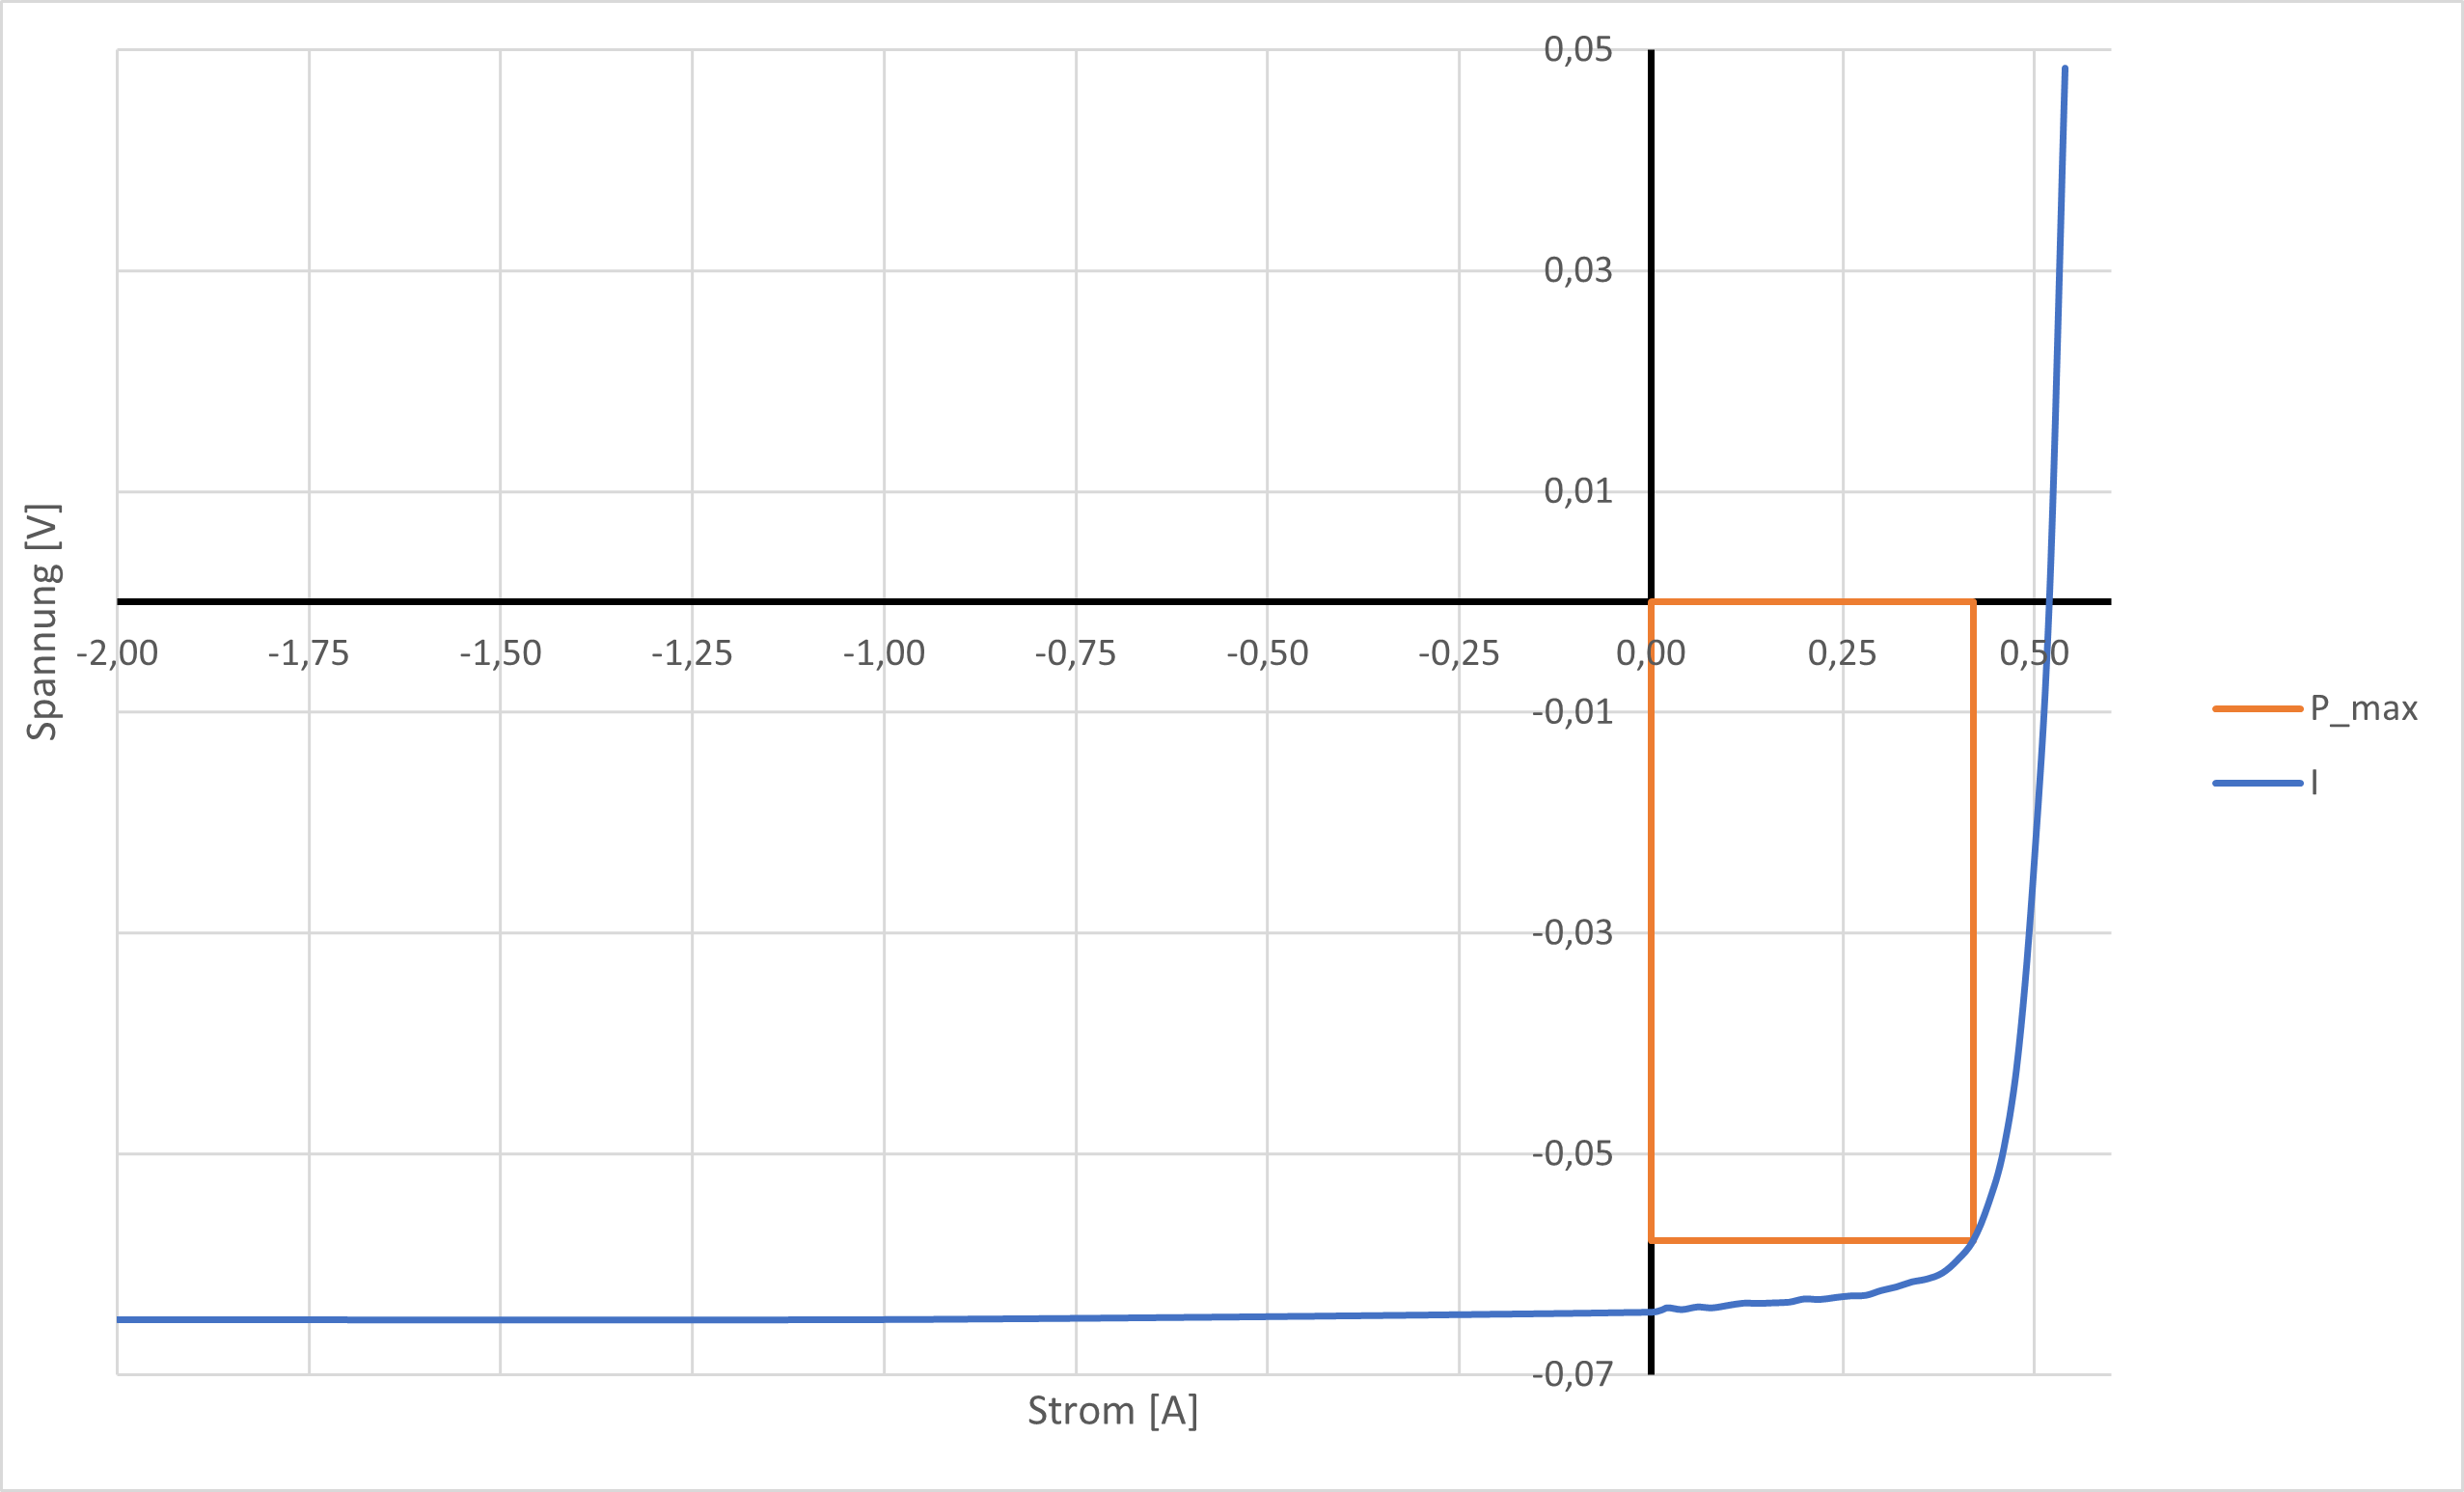
\includegraphics[width=14cm]{Diagramm_beleuchtet}
\centering
\caption{Diagramm Solarzelle unbeleuchtet}
\centering
\label{fig:beleuchtet}
\end{figure}

\newpage
\section{Literatur}
$[$1$]$ 


\label{LastPage}

\end{document}
%%% Local Variables:
%%% mode: latex
%%% TeX-master: t
%%% End:
